% ================================================================================
%
% Copyright (c) 2009, Nico Schlömer
% All rights reserved.
% 
% Redistribution and use in source and binary forms, with or without
% modification, are permitted provided that the following conditions are
% met:
% 
%     * Redistributions of source code must retain the above copyright
%       notice, this list of conditions and the following disclaimer.
%     * Redistributions in binary form must reproduce the above copyright
%       notice, this list of conditions and the following disclaimer in
%       the documentation and/or other materials provided with the distribution
% 
% THIS SOFTWARE IS PROVIDED BY THE COPYRIGHT HOLDERS AND CONTRIBUTORS "AS IS"
% AND ANY EXPRESS OR IMPLIED WARRANTIES, INCLUDING, BUT NOT LIMITED TO, THE
% IMPLIED WARRANTIES OF MERCHANTABILITY AND FITNESS FOR A PARTICULAR PURPOSE
% ARE DISCLAIMED. IN NO EVENT SHALL THE COPYRIGHT OWNER OR CONTRIBUTORS BE
% LIABLE FOR ANY DIRECT, INDIRECT, INCIDENTAL, SPECIAL, EXEMPLARY, OR
% CONSEQUENTIAL DAMAGES (INCLUDING, BUT NOT LIMITED TO, PROCUREMENT OF
% SUBSTITUTE GOODS OR SERVICES; LOSS OF USE, DATA, OR PROFITS; OR BUSINESS
% INTERRUPTION) HOWEVER CAUSED AND ON ANY THEORY OF LIABILITY, WHETHER IN
% CONTRACT, STRICT LIABILITY, OR TORT (INCLUDING NEGLIGENCE OR OTHERWISE)
% ARISING IN ANY WAY OUT OF THE USE OF THIS SOFTWARE, EVEN IF ADVISED OF THE
% POSSIBILITY OF SUCH DAMAGE.
%
% ================================================================================
\newpage
\section*{{\matlab} alternatives}
\addcontentsline{toc}{section}{{\matlab} alternatives}

When writing {\matlab} code, you need to realize that unlike C, Fortran, or Python code, you'll always need the \emph{commercial} {\matlab} environment to have it run. Right now, that might not be much of a problem to you as you are at a university or have some other free access to the software, but sometime in the future, this might change.

The current cost for the basic {\matlab} kit, which does not include \emph{any} toolbox nor Simulink, is \EUR{500} for academic institutions; around \EUR{60} for students; \emph{thousands} of Euros for commercial operations. Considering this, there is a not too small chance that you will not be able to legally use {\matlab} after you quit from university, and that would render all your code virtually useless to you.

Because of that, free and open source {\matlab} alternatives have emerged in recent years, two of which are shortly introduced here. Both of them try to stick to {\matlab} syntax as closely as possible, resulting in all of the code in this document being legal for the two packages as well. When it comes to the specialized toolboxes, however, they may not be able to provide the same capabilities that {\matlab} offers. Also note that neither Octave nor Scilab ship with their own text editors (as {\matlab} does), so you are free yo use the editor of your choice (see, for example, \href{http://www.vim.org/}{vim}, \href{http://www.gnu.org/software/emacs/}{emacs}, Kate, \href{http://projects.gnome.org/gedit/}{gedit} for Linux; \href{http://notepad-plus.sourceforge.net/uk/site.htm}{Notepad++}, \href{http://www.crimsoneditor.com/}{Crimson Editor} for Windows).

\subsection{GNU Octave}

\begin{floatingfigure}[r]{5cm}
\centering
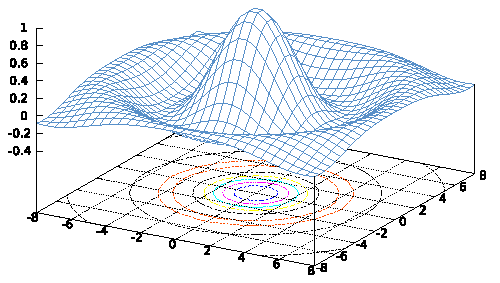
\includegraphics[width=5cm]{figures/Octave_Sombrero}
\end{floatingfigure}

GNU Octave is a high-level language, primarily intended for numerical computations. It provides a convenient command line interface for solving linear and nonlinear problems numerically, and for performing other numerical experiments using a language that is mostly compatible with {\matlab}. It may also be used as a batch-oriented language.

Internally, Octave relies on other independent and well-recognized packages such as gnuplot (for plotting) or UMFPACK (for calculating with sparse matrices). In that sense, Octave is extremely well integrated into the free and open source software (FOSS) landscape.

Octave has extensive tools for solving common numerical linear algebra problems, finding the roots of nonlinear equations, integrating ordinary functions, manipulating polynomials, and integrating ordinary differential and differential-algebraic equations. It is easily extensible and customizable via user-defined functions written in Octave's own language, or using dynamically loaded modules written in C++, C, Fortran, or other languages.

GNU Octave is also freely redistributable software. You may redistribute it and/or modify it under the terms of the GNU General Public License (GPL) as published by the Free Software Foundation.

The project if originally GNU/Linux, but versions for MacOS, Windows, Sun Solaris, and OS/2 exist.

\subsection{Scilab}

\begin{floatingfigure}[r]{4cm}
\centering

\includegraphics[width=4cm]{figures/scilab_official_logo}
\end{floatingfigure}

Scilab is a scientific software package for numerical computations providing a powerful open computing environment for engineering and scientific applications.

Scilab is open source software and originates from the French International Institute for Research in Computer Science and Control (INRIA).

Since 1994 it has been distributed freely along with the source code via the Internet. It is currently used in educational and industrial environments around the world.

Scilab is now the responsibility of the Scilab Consortium, launched in May 2003. There are currently 18 members in Scilab Consortium (Phase II).

Scilab includes hundreds of mathematical functions with the possibility to add interactively programs from various languages (C, C++, Fortran,\dots). It has sophisticated data structures (including lists, polynomials, rational functions, linear systems\dots), an interpreter and a high level programming language.

Scilab works under Windows 9X/2000/XP/Vista, GNU/Linux, and most UNIX systems. Binary versions for these systems are freely available, along with the source code.